% Source: graduate-coursework/Research/Intro_to_Agents/handouts/Part4_Planning_Workflow.tex

\documentclass[border=4pt]{standalone}
\usepackage{graphicx}
\usepackage{tikz}
\usepackage{xcolor}
\usetikzlibrary{shapes.geometric, arrows.meta, positioning, calc, fit, backgrounds}

\definecolor{UofSCGarnet}{HTML}{73000A}
\definecolor{UofSCBlack}{HTML}{000000}
\definecolor{UofSCWhite}{HTML}{FFFFFF}
\definecolor{UofSCAtlantic}{HTML}{466A9F}
\definecolor{UofSCCongaree}{HTML}{1F414D}
\definecolor{UofSCHorseshoe}{HTML}{65780B}
\definecolor{UofSCRose}{HTML}{CC2E40}
\definecolor{UofSCDarkGarnet}{HTML}{570008}
\definecolor{UofSC90Black}{HTML}{363636}
\definecolor{UofSC70Black}{HTML}{5C5C5C}
\definecolor{UofSC50Black}{HTML}{A2A2A2}

\tikzset{
    box/.style={
        draw=UofSCBlack,
        fill=#1,
        minimum width=2.5cm,
        minimum height=0.8cm,
        text=UofSCWhite,
        font=\small\bfseries,
        align=center,
        inner sep=4pt
    },
    box/.default=UofSCGarnet,
    lightbox/.style={
        draw=UofSCBlack,
        fill=UofSCWhite,
        minimum width=2.5cm,
        minimum height=0.8cm,
        text=UofSCBlack,
        font=\small,
        align=center,
        inner sep=4pt
    },
    arrow/.style={
        ->,
        >=Stealth,
        thick,
        UofSCBlack
    },
    bigarrow/.style={
        ->,
        >=Stealth,
        line width=1.5pt,
        UofSCGarnet
    },
    phase/.style={
        draw=UofSCBlack,
        fill=#1,
        minimum width=3cm,
        minimum height=1cm,
        text=UofSCWhite,
        font=\bfseries,
        align=center
    },
    phase/.default=UofSCGarnet,
    subphase/.style={
        draw=UofSC70Black,
        fill=UofSCWhite,
        minimum width=2.8cm,
        minimum height=0.6cm,
        text=UofSCBlack,
        font=\scriptsize,
        align=center
    },
    cyclebox/.style={
        draw=UofSCBlack,
        line width=1.5pt,
        fill=#1,
        minimum width=2cm,
        minimum height=1.2cm,
        text=UofSCWhite,
        font=\bfseries,
        align=center
    },
    cyclebox/.default=UofSCGarnet
}

\begin{document}
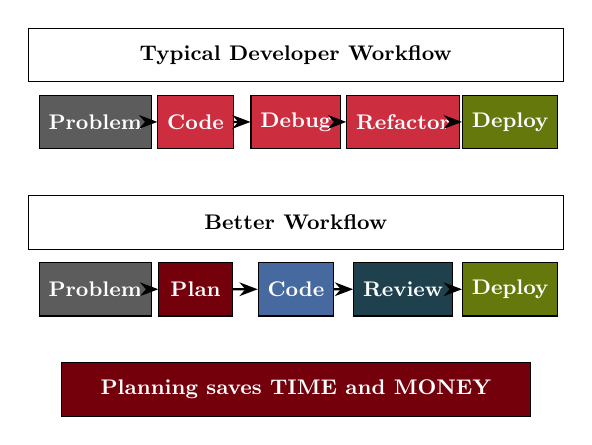
\begin{tikzpicture}[node distance=0.4cm, scale=0.85, transform shape]
                % Typical workflow
                \node[lightbox, minimum width=8cm, minimum height=0.8cm] (typical) at (0,2) {\textbf{Typical Developer Workflow}};
                \node[box=UofSC70Black, minimum width=1.3cm] (p1) at (-3,1) {Problem};
                \node[box=UofSCRose, minimum width=1.1cm] (c1) at (-1.5,1) {Code};
                \node[box=UofSCRose, minimum width=1.1cm] (d1) at (0,1) {Debug};
                \node[box=UofSCRose, minimum width=1.3cm] (r1) at (1.6,1) {Refactor};
                \node[box=UofSCHorseshoe, minimum width=1.1cm] (dep1) at (3.2,1) {Deploy};

                \draw[arrow] (p1) -- (c1);
                \draw[arrow] (c1) -- (d1);
                \draw[arrow] (d1) -- (r1);
                \draw[arrow] (r1) -- (dep1);

                % Better workflow
                \node[lightbox, minimum width=8cm, minimum height=0.8cm] (better) at (0,-0.5) {\textbf{Better Workflow}};
                \node[box=UofSC70Black, minimum width=1.3cm] (p2) at (-3,-1.5) {Problem};
                \node[box=UofSCGarnet, minimum width=1.1cm] (plan) at (-1.5,-1.5) {Plan};
                \node[box=UofSCAtlantic, minimum width=1.1cm] (c2) at (0,-1.5) {Code};
                \node[box=UofSCCongaree, minimum width=1.1cm] (rev) at (1.6,-1.5) {Review};
                \node[box=UofSCHorseshoe, minimum width=1.1cm] (dep2) at (3.2,-1.5) {Deploy};

                \draw[arrow] (p2) -- (plan);
                \draw[arrow] (plan) -- (c2);
                \draw[arrow] (c2) -- (rev);
                \draw[arrow] (rev) -- (dep2);

                % Result box
                \node[box=UofSCGarnet, minimum width=7cm, minimum height=0.8cm, text width=6.5cm] at (0,-3) {Planning saves TIME and MONEY};
            \end{tikzpicture}
\end{document}
